\chapter{Contatori Elettronici}
I \textbf{contatori elettronici} vengono usati per convertire una \textbf{grandezza analogica} in un \textbf{valore numerico}, attraverso la tecnica del \textbf{conteggio}.\\ \\
Possono misurare:
\begin{itemize}
    \item Eventi
    \item Periodi
    \item Frequenze
    \item Intervalli di tempo
    \item ...
\end{itemize}
Si basano su una serie di \textbf{blocchi connessi} che andremo qui a vedere.
\section{Blocchi}
\subsection{Blocco di Ingresso}
Questo blocco ha lo scopo di \textbf{condizionare} il segnale in ingresso per estrarre i valori destinati ai blocchi che lo seguono:
\begin{center}
    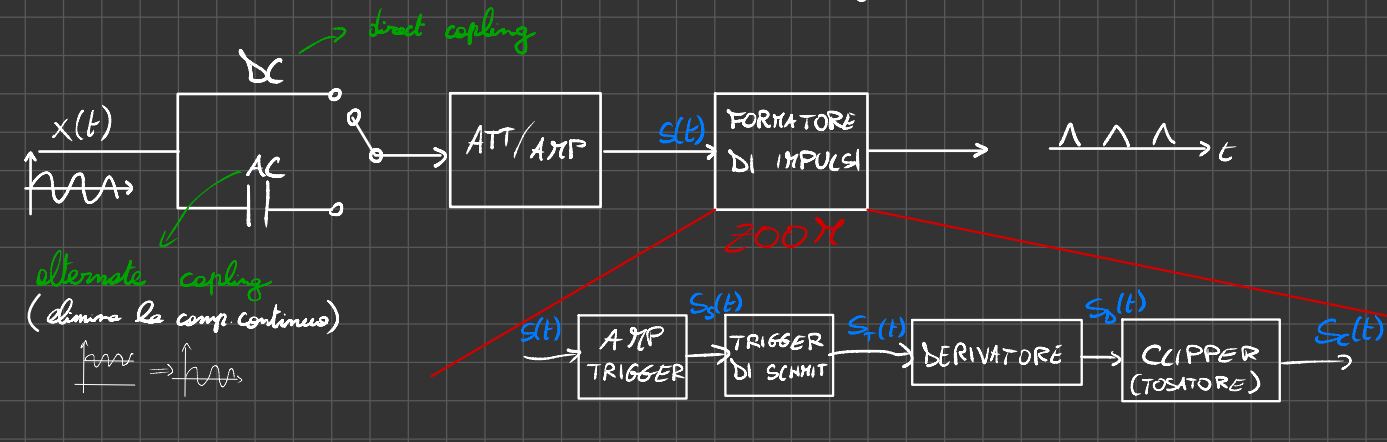
\includegraphics[width=\textwidth]{Images/figure7.png}
\end{center}
In particolare:
\begin{itemize}
    \item L'\textbf{Amplificatore di Trigger} manda in \textbf{saturazione} il segnale
    \item Il \textbf{Trigger di Smith} fa diventare il segnale \textbf{un'onda quadra}
    \item Il \textbf{derivatore} \textbf{deriva} il segnale che ha in ingresso, creando un \textbf{treno di impulsi}
    \item Il \textbf{tosatore} (o clipper) \textbf{elimina gli impulsi positivi o quelli negativi}
\end{itemize}
\subsection{Blocco di Gate}
Il blocco di \textbf{gate} è una sorta di \textbf{interruttore}, che decide gli \textbf{impulsi} \textbf{da} \textbf{contare}:
\begin{center}
    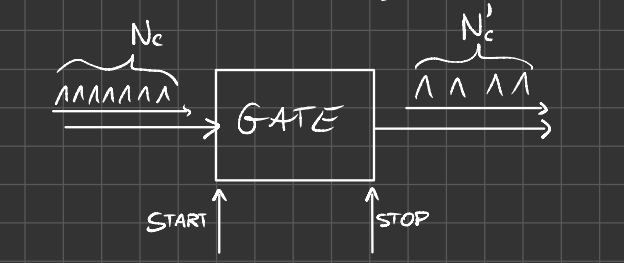
\includegraphics[width=.6\textwidth]{Images/figure8.png}
\end{center}
\subsection{Blocco di Conteggio}
Questo blocco esegue il \textbf{conteggio} \textbf{degli} \textbf{impulsi} compresi tra il segnale di \textbf{START} e quello di \textbf{STOP}, ed è formato da una serie di più \textbf{contatori elementari} di modulo m (generalmente m= 10):
\begin{center}
    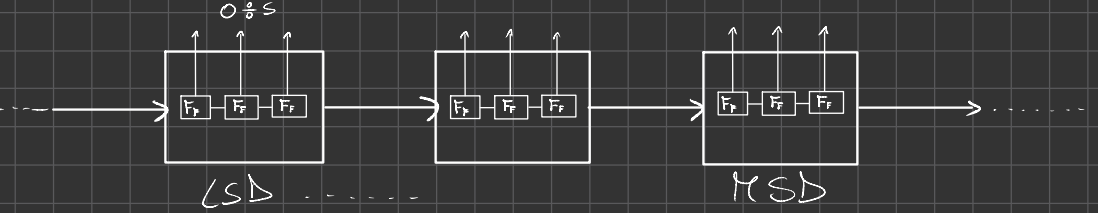
\includegraphics[width=.8\textwidth]{Images/figure9.png}
\end{center}
\subsection{Blocco di Visualizzazione}
Il \textbf{Latch} è un circuito di tenuta che riceve il risultato del conteggio e lo manda al \textbf{display}, omettendo così variazioni rapide del risultato.
\begin{center}
    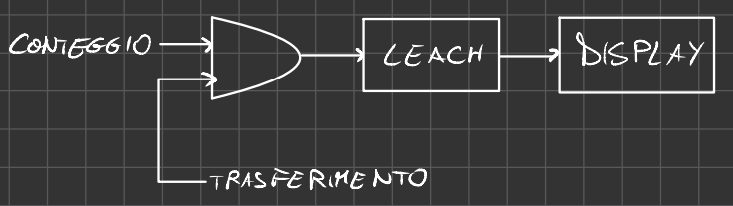
\includegraphics[width=.8\textwidth]{Images/figure10.png}
\end{center}
\subsection{Oscillatore di Riferimento}
\textbf{L'oscillatore di riferimento} è l'elemento fondante per misurare \textbf{tempi}, \textbf{periodi}, \textbf{frequenze}, etc.
\section{Contatore di Eventi}
\begin{center}
    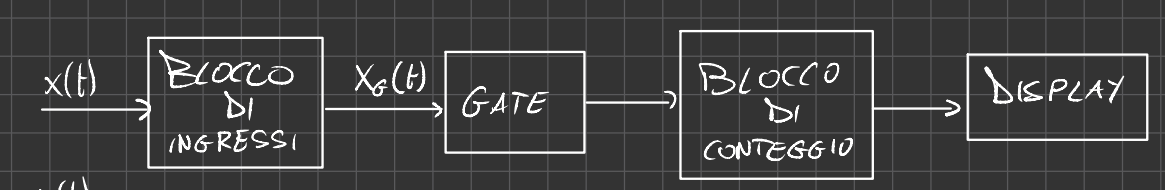
\includegraphics[width=\textwidth]{Images/figure11.png}
\end{center}
\section{Misure di Periodo}
\begin{center}
    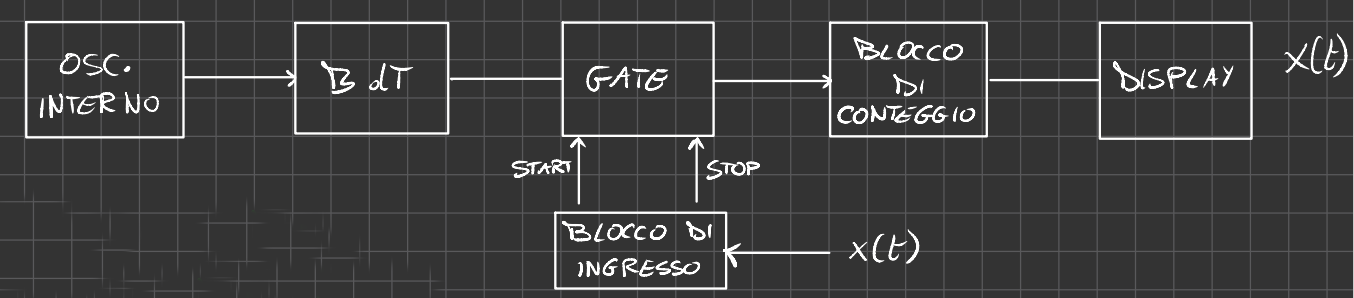
\includegraphics[width=\textwidth]{Images/figure13.png}
\end{center}
In questo caso \textbf{START} e \textbf{STOP} sono dati dal segnale di ingresso e $T_x$ corrisponde a $T_{on}$, in particolare:
\begin{equation*}
    T_x = T_{on} = N_c \cdot T_c
\end{equation*}
Dove $N_c$ sono i numeri di \textbf{impulsi di clock} e $T_c$ è il \textbf{periodo di clock}.\\ \\
In questo caso:
\begin{equation*}
    \Delta T_x = T_c \ e \ \Gamma_{T_x} = \frac{\Delta T_x}{T_x} = \frac{T_c}{N_x T_C} = \frac{1}{N_x}
\end{equation*}
\section{Misure di Frequenza}
\begin{center}
    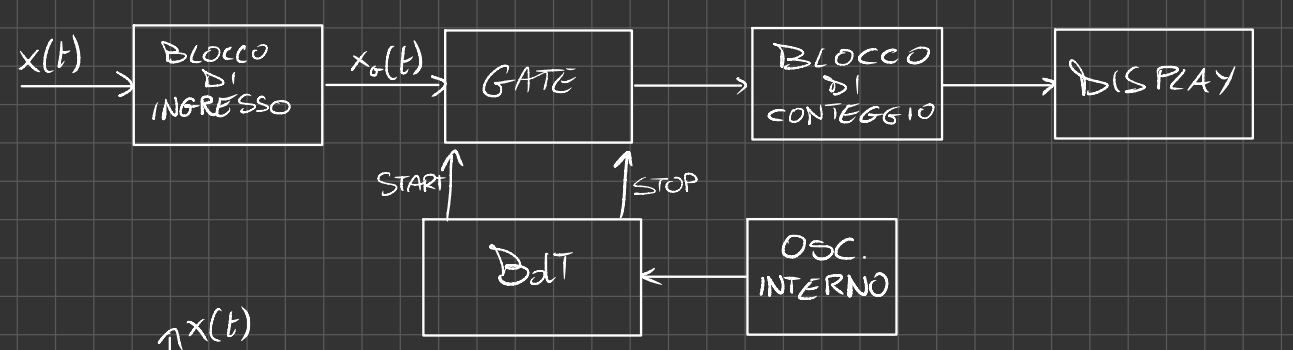
\includegraphics[width=\textwidth]{Images/figure12.png}
\end{center}
Indichiamo con:
\begin{itemize}
    \item $T_{on}$ il lasso di tempo che va tra \textbf{START} e \textbf{STOP}
    \item $N_x$ il numero di impulsi(periodi in questo caso) contati
    \item $T_x$ il periodo che va tra un impulso e l'altro
\end{itemize}
Quindi avremo che:
\begin{equation*}
    T_{on} =\footnote{a meno della quantizzazione} N_x T_x \implies F_x = \frac{N_x}{T_{on}}
\end{equation*}
E che La \textbf{risoluzione} \textbf{assoluta} sia:
\begin{equation*}
    \Delta F_x = \frac{1}{T_{on}} \quad con \quad N_x = 1
\end{equation*}
E che:
\begin{equation*}
    \Gamma_{F_x} = \frac{\Delta F_x}{F_x} = \frac{1}{T_{on} \frac{N_x}{T_{on}}} = \frac{1}{N_x}
\end{equation*}

\section{Incertezza dovuta al Trigger}
La principale componente di incertezza dovuta al trigger, viene detto \textbf{Trigger Level Error}, che nasce nelle misure di \textbf{intervalli di tempo}, quando le pendenze dei segnali di \textbf{START} e di \textbf{STOP} non sono le stesse.\\ \\
Un'ulteriore componente di incertezza è dovuta al \textbf{rumore} sovrapposto al segnale e viene detto \textbf{Trigger Level Timing Error}.